\documentclass[10pt]{article}

\usepackage[a4paper,margin=0.65in]{geometry}
\usepackage{amsmath,amssymb}
\usepackage{graphicx}
\usepackage{booktabs}
\usepackage{array}
\usepackage{float}
\usepackage{hyperref}
\usepackage{enumitem}
\usepackage{xcolor}
\usepackage[font=small]{caption}
\graphicspath{{figs/}}
\newcommand{\fig}[3]{\begin{figure}[H]\centering\includegraphics[width=#2\linewidth]{#1}\caption{#3}\end{figure}}
\newcommand{\figpair}[3]{\begin{figure}[H]\centering\includegraphics[width=0.485\linewidth]{#1}\hfill\includegraphics[width=0.485\linewidth]{#2}\caption{#3}\end{figure}}
\newcommand{\inference}[4]{\textbf{Inference.} \emph{What the plot shows:} #1 \emph{Trend observed:} #2 \emph{Why it occurs:} #3 \emph{Conclusion:} #4}
\usepackage{tikz}
\usetikzlibrary{positioning,arrows.meta,shapes.geometric,fit,calc}

\setlist{nosep,leftmargin=*}
\renewcommand{\arraystretch}{1.2}
\setlength{\parindent}{0pt}
\setlength{\parskip}{2pt}

\tikzset{
layer/.style={
draw,
rounded corners,
minimum width=1.7cm,
minimum height=0.65cm,
align=center,
fill=blue!10,
font=\scriptsize
},
smalllayer/.style={
draw,
rounded corners,
minimum width=1.35cm,
minimum height=0.58cm,
align=center,
fill=green!10,
font=\scriptsize
},
arrow/.style={
-{Latex[length=2mm]},
thin
}
}

\begin{document}

%%%%%%%%%%%%%%%%%%%%%%%%%%%%%%%%%%%%%%%%%%%%%%%%%%%%%%%%%%%%
% TITLE
%%%%%%%%%%%%%%%%%%%%%%%%%%%%%%%%%%%%%%%%%%%%%%%%%%%%%%%%%%%%

\begin{center}

{\large\textbf{Shiv Nadar University Chennai}}

\vspace{2mm}

{\normalsize\textbf{CS3807 -- Deep Learning Laboratory}}

\vspace{2mm}

{\large\textbf{Experiment 7}}

\vspace{1mm}

{\normalsize\textbf{End-to-End Study of Autoencoders, Convolutional}}

{\normalsize\textbf{Autoencoders, Denoising Autoencoders and Variational Autoencoders}}

\end{center}


\textbf{Repository Link:}
\textbf{\url{https://github.com/Atharsh2910/Deep_Learning_Lab/tree/main/Lab7}
}


\vspace{3mm}

\begin{tabular}{|p{3.8cm}|p{8cm}|p{2cm}|}
\hline
Degree \& Branch & B.Tech Artificial Intelligence \& Data Science & Semester V\\ \hline
Subject Code \& Name & CS3807 -- Deep Learning Laboratory & AY: 2026--27\\ \hline
\end{tabular}

\begin{tabular}{|p{3.5cm}|p{8cm}|}
\hline
\textbf{Name} & {ATHARSH S U}\\ \hline
\textbf{Register Number} &{24011101008} \\ \hline
\textbf{Roll Number} &{24110049} \\ \hline
\textbf{Class} & {AI-DS 'A'}\\ \hline
\end{tabular}
\vspace{3mm}

%%%%%%%%%%%%%%%%%%%%%%%%%%%%%%%%%%%%%%%%%%%%%%%%%%%%%%%%%%%%
\section*{1. Objective}

The objective of this experiment is to develop an end-to-end understanding of
autoencoders and their variants for image representation, reconstruction,
denoising and generative modeling.

The experiment begins with a fully connected autoencoder, progresses to a
Convolutional Autoencoder (CAE), introduces image corruption for denoising,
and finally develops a Variational Autoencoder (VAE). Students will visualize
the learned latent representation, compare reconstruction quality using
quantitative and qualitative measures, and explore the generative capability
of the VAE.

The same image dataset and a controlled experimental protocol should be used
throughout the experiment wherever possible.

%%%%%%%%%%%%%%%%%%%%%%%%%%%%%%%%%%%%%%%%%%%%%%%%%%%%%%%%%%%%
\section*{2. Learning Outcomes}

After completing this experiment, students will be able to:

\begin{itemize}
\item explain the encoder--latent--decoder structure of an autoencoder;
\item prepare image data for reconstruction-based learning;
\item implement a fully connected autoencoder;
\item implement a Convolutional Autoencoder for image reconstruction;
\item introduce controlled noise and build a denoising autoencoder;
\item evaluate reconstruction using MSE, MAE and SSIM;
\item visualize and interpret latent representations;
\item explain the probabilistic latent representation of a VAE;
\item implement the reparameterization trick;
\item calculate and interpret reconstruction and KL-divergence losses;
\item generate new images by sampling from a learned latent space; and
\item compare deterministic and variational latent representations.
\end{itemize}

%%%%%%%%%%%%%%%%%%%%%%%%%%%%%%%%%%%%%%%%%%%%%%%%%%%%%%%%%%%%
\section*{3. Dataset and Experimental Setup}

\textbf{Dataset: MNIST Handwritten Digit Dataset}

MNIST contains grayscale images of handwritten digits from 0 to 9. Each image
has spatial dimensions

\[
28\times28\times1.
\]

The dataset is particularly suitable for this experiment because the images
are small, the classes have visually meaningful structure, and the same image
format can be directly supplied to fully connected, convolutional and
variational autoencoders.

The dataset can be loaded directly using Keras/TensorFlow:

\url{https://www.tensorflow.org/api_docs/python/tf/keras/datasets/mnist}

\textbf{Recommended laboratory subset:}

Use 10,000 training images and 2,000 test images for the main laboratory
execution. The full MNIST dataset may be used if computational resources
permit.

The labels are not required as reconstruction targets. The original image is
the target:

\[
\boxed{x\rightarrow \text{Encoder}\rightarrow z
\rightarrow\text{Decoder}\rightarrow\hat{x}}
\]

where $x$ is the input image and $\hat{x}$ is its reconstruction.

\textbf{Setup used in this execution:} the first 10,000 MNIST training
images were used, of which 9,000 form the training set and 1,000 (10\%) form the
validation set, together with the first 2,000 MNIST test images. The resulting
shapes are $(9000,28,28,1)$ for training, $(1000,28,28,1)$ for validation and
$(2000,28,28,1)$ for testing; the pixel range is $0$--$1$ and the flattened
input of the FC model has shape $(9000,784)$. All runs used random seed 42,
TensorFlow 2.20.0 with Keras 3.13.2, on a Kaggle GPU (Tesla T4 $\times$ 2).

\fig{mnist_samples}{0.9}{MNIST training samples, normalised to $[0,1]$.}

%%%%%%%%%%%%%%%%%%%%%%%%%%%%%%%%%%%%%%%%%%%%%%%%%%%%%%%%%%%%
\section*{4. Expected Input and Output}

\subsection*{Expected Input}

Each input image has shape

\[
28\times28\times1.
\]

For a batch of 32 images:

\[
X\in\mathbb{R}^{32\times28\times28\times1}.
\]

Pixel values should be converted from

\[
[0,255]\rightarrow[0,1].
\]

For a fully connected autoencoder, the image may be flattened:

\[
28\times28=784.
\]

Therefore,

\[
x\in\mathbb{R}^{784}.
\]

For a convolutional autoencoder, retain the spatial structure:

\[
x\in\mathbb{R}^{28\times28\times1}.
\]

\subsection*{Expected Output}

The primary output is a reconstructed image:

\[
\hat{x}\in\mathbb{R}^{28\times28\times1}.
\]

Students must display:

\begin{verbatim}
Original image
Reconstructed image
Reconstruction error
\end{verbatim}

For the denoising model, display:

\begin{verbatim}
Original clean image
Noisy image
Denoised reconstruction
\end{verbatim}

For the VAE, display newly generated samples obtained by sampling from the
latent distribution.

%%%%%%%%%%%%%%%%%%%%%%%%%%%%%%%%%%%%%%%%%%%%%%%%%%%%%%%%%%%%
\section*{5. Overall Experimental Pipeline}

The complete experiment follows:

\begin{center}
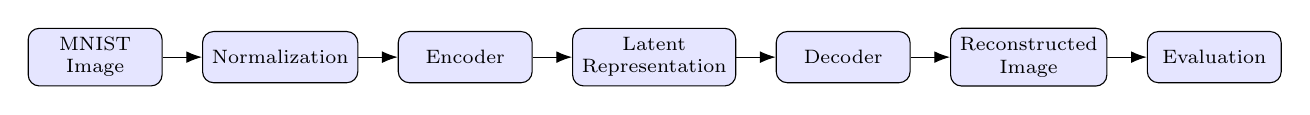
\begin{tikzpicture}[node distance=5mm]
\node[layer](a){MNIST\\Image};
\node[layer,right=of a](b){Normalization};
\node[layer,right=of b](c){Encoder};
\node[layer,right=of c](d){Latent\\Representation};
\node[layer,right=of d](e){Decoder};
\node[layer,right=of e](f){Reconstructed\\Image};
\node[layer,right=of f](g){Evaluation};

\foreach \x/\y in {a/b,b/c,c/d,d/e,e/f,f/g}
\draw[arrow](\x)--(\y);
\end{tikzpicture}
\end{center}

The experiment consists of four related studies:

\begin{enumerate}
\item Fully Connected Autoencoder
\item Convolutional Autoencoder
\item Denoising Convolutional Autoencoder
\item Variational Autoencoder
\end{enumerate}

%%%%%%%%%%%%%%%%%%%%%%%%%%%%%%%%%%%%%%%%%%%%%%%%%%%%%%%%%%%%
\section*{6. Exploring Autoencoders}

An autoencoder learns to reproduce its input at the output.

The encoder maps the input to a lower-dimensional representation:

\[
z=f_{\theta}(x),
\]

and the decoder reconstructs the input:

\[
\hat{x}=g_{\phi}(z).
\]

The training objective is to minimize reconstruction error:

\[
\mathcal{L}_{rec}
=
\frac{1}{N}\sum_{i=1}^{N}
\|x_i-\hat{x}_i\|^2.
\]

\begin{center}
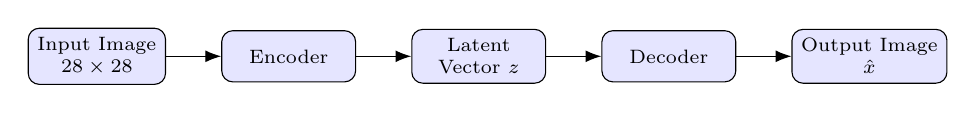
\begin{tikzpicture}[node distance=7mm]
\node[layer](a){Input Image\\$28\times28$};
\node[layer,right=of a](b){Encoder};
\node[layer,right=of b](c){Latent\\Vector $z$};
\node[layer,right=of c](d){Decoder};
\node[layer,right=of d](e){Output Image\\$\hat{x}$};

\foreach \x/\y in {a/b,b/c,c/d,d/e}
\draw[arrow](\x)--(\y);
\end{tikzpicture}
\end{center}

The latent vector is a compressed representation of the input.

%%%%%%%%%%%%%%%%%%%%%%%%%%%%%%%%%%%%%%%%%%%%%%%%%%%%%%%%%%%%
\section*{7. Fully Connected Autoencoder}

Flatten each image from

\[
28\times28=784
\]

to a vector of length 784.

Use the following architecture:

\begin{center}
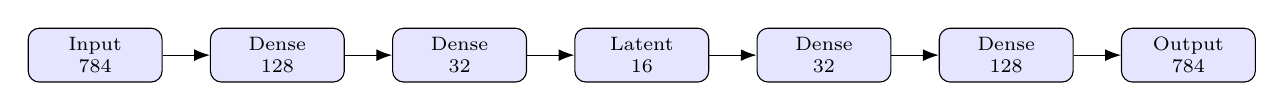
\begin{tikzpicture}[node distance=6mm]
\node[layer](a){Input\\784};
\node[layer,right=of a](b){Dense\\128};
\node[layer,right=of b](c){Dense\\32};
\node[layer,right=of c](d){Latent\\16};
\node[layer,right=of d](e){Dense\\32};
\node[layer,right=of e](f){Dense\\128};
\node[layer,right=of f](g){Output\\784};

\foreach \x/\y in {a/b,b/c,c/d,d/e,e/f,f/g}
\draw[arrow](\x)--(\y);
\end{tikzpicture}
\end{center}

Use ReLU activation in hidden layers and sigmoid activation in the output
layer.

\textbf{Suggested configuration:}

\begin{center}
\begin{tabular}{|l|l|}
\hline
Parameter & Value\\
\hline
Latent dimension & 16\\
Optimizer & Adam\\
Learning rate & $10^{-3}$\\
Batch size & 128\\
Epochs & 20\\
Loss & Binary Cross-Entropy\\
\hline
\end{tabular}
\end{center}

The encoder has 105,136 parameters, the decoder 105,904, and the complete
FC autoencoder has 211,040 trainable parameters. The latent layer itself has no
activation. Training time for 20 epochs was 11.0\,s.

%%%%%%%%%%%%%%%%%%%%%%%%%%%%%%%%%%%%%%%%%%%%%%%%%%%%%%%%%%%%
\section*{8. Required Analysis of the Basic Autoencoder}

\textbf{Plot 1: Original versus Reconstructed Images}

\fig{plot1_original_vs_recon_fc}{0.85}{Plot 1: Original, FC-AE reconstruction ($d_z=16$) and absolute-error map for ten test images.}


\textbf{Plot 2: Training and Validation Reconstruction Loss}

\begin{itemize}
\item X-axis: Epoch
\item Y-axis: Reconstruction loss
\item Curves: Training loss and validation loss
\end{itemize}

\fig{plot2_fc_loss}{0.55}{Plot 2: FC-AE training and validation reconstruction loss (binary cross-entropy) versus epoch.}


%%%%%%%%%%%%%%%%%%%%%%%%%%%%%%%%%%%%%%%%%%%%%%%%%%%%%%%%%%%%
\section*{9. Reconstruction Metrics}

Students must calculate the following metrics on the test set.

\subsection*{Mean Squared Error}

\[
MSE=
\frac{1}{N}
\sum_{i=1}^{N}
(x_i-\hat{x}_i)^2.
\]

\subsection*{Mean Absolute Error}

\[
MAE=
\frac{1}{N}
\sum_{i=1}^{N}
|x_i-\hat{x}_i|.
\]

\subsection*{Structural Similarity}

Calculate SSIM between the original and reconstructed images.

The implementation may use:

\url{https://scikit-image.org/docs/stable/api/skimage.metrics.html}

Report:

\begin{center}
\begin{tabular}{|l|c|}
\hline
Metric & Value\\
\hline
Test MSE & 0.02046\\
Test MAE & 0.05514\\
Mean SSIM & 0.75857\\
\hline
\end{tabular}
\end{center}

%%%%%%%%%%%%%%%%%%%%%%%%%%%%%%%%%%%%%%%%%%%%%%%%%%%%%%%%%%%%
\section*{10. Convolutional Autoencoder}

A Convolutional Autoencoder preserves spatial structure and uses convolutional
operations in the encoder and upsampling/transposed convolution operations
in the decoder.

The conceptual architecture is:

\begin{center}
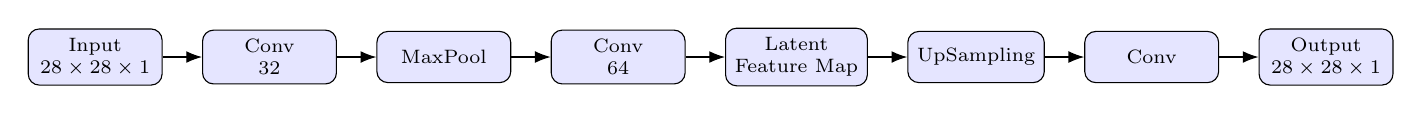
\begin{tikzpicture}[node distance=5mm]
\node[layer](a){Input\\$28\times28\times1$};
\node[layer,right=of a](b){Conv\\32};
\node[layer,right=of b](c){MaxPool};
\node[layer,right=of c](d){Conv\\64};
\node[layer,right=of d](e){Latent\\Feature Map};
\node[layer,right=of e](f){UpSampling};
\node[layer,right=of f](g){Conv};
\node[layer,right=of g](h){Output\\$28\times28\times1$};

\foreach \x/\y in {a/b,b/c,c/d,d/e,e/f,f/g,g/h}
\draw[arrow](\x)--(\y);
\end{tikzpicture}
\end{center}


\fig{cae_loss}{0.55}{CAE training and validation reconstruction loss (binary cross-entropy).}

Final training loss 0.0681, final validation loss 0.0694, gap 0.0013; the best
validation epoch is 20/20 and the validation loss changed by 0.76\% over the
last three epochs, i.e.\ the CAE is converging/near a plateau with no clear
overfitting.

%%%%%%%%%%%%%%%%%%%%%%%%%%%%%%%%%%%%%%%%%%%%%%%%%%%%%%%%%%%%
\section*{11. Comparing Fully Connected and Convolutional Autoencoders}

Train both models using the same training and test images.

\begin{center}
\begin{tabular}{|l|c|c|c|c|}
\hline
Model & MSE & MAE & SSIM & Parameters\\
\hline
Fully Connected AE & 0.02046 & 0.05514 & 0.75857 & 211,040\\
Convolutional AE & 0.00259 & 0.01500 & 0.97395 & 74,497\\
\hline
\end{tabular}
\end{center}

\textbf{Plot 3: Reconstruction Comparison}

Display:

\[
\text{Original}
\rightarrow
\text{FC-AE Reconstruction}
\rightarrow
\text{CAE Reconstruction}.
\]

\fig{plot3_fc_vs_cae}{0.85}{Plot 3: Original $\rightarrow$ FC-AE $\rightarrow$ CAE reconstructions with the corresponding absolute-error maps.}



%%%%%%%%%%%%%%%%%%%%%%%%%%%%%%%%%%%%%%%%%%%%%%%%%%%%%%%%%%%%
\section*{12. Denoising Autoencoder}

A denoising autoencoder receives a corrupted image but is trained to
reconstruct the original clean image.

The training mapping is:

\[
\boxed{\tilde{x}\rightarrow\text{Encoder}\rightarrow z
\rightarrow\text{Decoder}\rightarrow\hat{x}}
\]

where $\tilde{x}$ is a noisy version of the clean image $x$.

\begin{center}
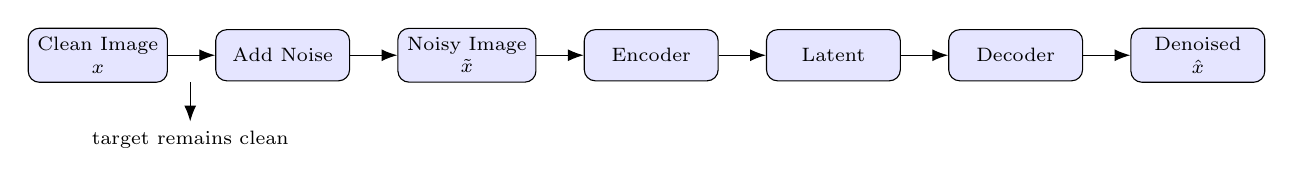
\begin{tikzpicture}[node distance=6mm]
\node[layer](a){Clean Image\\$x$};
\node[layer,right=of a](b){Add Noise};
\node[layer,right=of b](c){Noisy Image\\$\tilde{x}$};
\node[layer,right=of c](d){Encoder};
\node[layer,right=of d](e){Latent};
\node[layer,right=of e](f){Decoder};
\node[layer,right=of f](g){Denoised\\$\hat{x}$};

\foreach \x/\y in {a/b,b/c,c/d,d/e,e/f,f/g}
\draw[arrow](\x)--(\y);

\draw[arrow]($(a.south)!0.5!(b.south)$) -- ++(0,-5mm)
node[below,font=\scriptsize]{target remains clean};
\end{tikzpicture}
\end{center}

%%%%%%%%%%%%%%%%%%%%%%%%%%%%%%%%%%%%%%%%%%%%%%%%%%%%%%%%%%%%
\section*{13. Adding Image Noise}

Use at least two corruption types.

\subsection*{Gaussian Noise}

\[
\tilde{x}=x+n,
\qquad
n\sim\mathcal{N}(0,\sigma^2).
\]

Suggested standard deviations:

\[
\sigma\in\{0.1,0.2,0.3\}.
\]

Clip the resulting image to the range $[0,1]$.

\subsection*{Salt-and-Pepper Noise}

Randomly replace a small proportion of pixels with values close to 0 or 1.

Suggested corruption levels:

\[
p\in\{0.05,0.10,0.20\}.
\]

%%%%%%%%%%%%%%%%%%%%%%%%%%%%%%%%%%%%%%%%%%%%%%%%%%%%%%%%%%%%
\section*{14. Required Denoising Plots}

\textbf{Plot 4: Clean vs. Noisy vs. Denoised}

For at least 10 images, display:

\[
\text{Clean}\quad|\quad
\text{Noisy}\quad|\quad
\text{Denoised}.
\]

\fig{plot4_gauss_0.2}{0.85}{Plot 4: Clean $|$ Noisy $|$ Denoised for ten test images (Gaussian noise, $\sigma=0.2$), with absolute error of the denoised output.}
\fig{plot4_gauss_0.3}{0.85}{Plot 4 (continued): Gaussian noise, $\sigma=0.3$.}
\fig{plot4_sp_0.1}{0.85}{Plot 4 (continued): salt-and-pepper noise, $p=0.10$.}

\textbf{Plot 5: Noise Level vs. Reconstruction Quality}

For each noise level, calculate:

\[
MSE,\quad MAE,\quad SSIM.
\]

Report:

\begin{center}
\begin{tabular}{|c|c|c|c|}
\hline
Noise Level & MSE & MAE & SSIM\\
\hline
0.1 & 0.00340 & 0.01766 & 0.96089\\
0.2 & 0.00448 & 0.02091 & 0.94638\\
0.3 & 0.00653 & 0.02642 & 0.91534\\
\hline
\end{tabular}
\end{center}

\begin{center}
\begin{tabular}{|c|c|c|c|}
\hline
Noise Level ($p$, salt-and-pepper) & MSE & MAE & SSIM\\
\hline
0.05 & 0.00423 & 0.01953 & 0.95431\\
0.10 & 0.00506 & 0.02164 & 0.94335\\
0.20 & 0.00761 & 0.02759 & 0.90526\\
\hline
\end{tabular}
\end{center}

\begin{center}
\begin{tabular}{|l|c|c|c|c|}
\hline
Noisy input (before denoising) & Level & MSE & MAE & SSIM\\
\hline
Gaussian & 0.1 & 0.00543 & 0.04408 & 0.67892\\
Gaussian & 0.2 & 0.02122 & 0.08664 & 0.59385\\
Gaussian & 0.3 & 0.04666 & 0.12808 & 0.50938\\
Salt-and-pepper & 0.05 & 0.02406 & 0.02497 & 0.70834\\
Salt-and-pepper & 0.10 & 0.04830 & 0.05014 & 0.57743\\
Salt-and-pepper & 0.20 & 0.09585 & 0.09952 & 0.44776\\
\hline
\end{tabular}
\end{center}

\fig{plot5_noise_gaussian}{0.95}{Plot 5: Gaussian noise level versus MSE, MAE and SSIM (noisy input and denoised output).}
\fig{plot5_noise_saltpepper}{0.95}{Plot 5 (continued): salt-and-pepper noise level versus MSE, MAE and SSIM.}

\figpair{dcae_gauss_loss}{dcae_sp_loss}{Training and validation loss of the DCAE trained on Gaussian noise (left) and on salt-and-pepper noise (right).}



%%%%%%%%%%%%%%%%%%%%%%%%%%%%%%%%%%%%%%%%%%%%%%%%%%%%%%%%%%%%
\section*{15. Variational Autoencoder}

A conventional autoencoder maps an input to a deterministic latent vector:

\[
z=f(x).
\]

A VAE instead learns a probability distribution:

\[
q_{\phi}(z|x)
=
\mathcal{N}
\left(
\mu(x),
\operatorname{diag}(\sigma^2(x))
\right).
\]

The encoder produces:

\[
\mu,\qquad \log\sigma^2.
\]

A latent vector is sampled using the reparameterization trick:

\[
z=\mu+\sigma\odot\epsilon,
\qquad
\epsilon\sim\mathcal{N}(0,I).
\]

\begin{center}
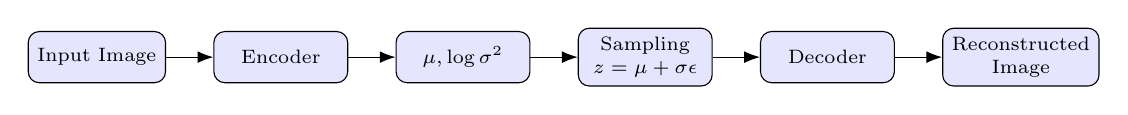
\begin{tikzpicture}[node distance=6mm]
\node[layer](a){Input Image};
\node[layer,right=of a](b){Encoder};
\node[layer,right=of b](c){$\mu,\log\sigma^2$};
\node[layer,right=of c](d){Sampling\\$z=\mu+\sigma\epsilon$};
\node[layer,right=of d](e){Decoder};
\node[layer,right=of e](f){Reconstructed\\Image};

\foreach \x/\y in {a/b,b/c,c/d,d/e,e/f}
\draw[arrow](\x)--(\y);
\end{tikzpicture}
\end{center}

%%%%%%%%%%%%%%%%%%%%%%%%%%%%%%%%%%%%%%%%%%%%%%%%%%%%%%%%%%%%
\section*{16. VAE Loss Function}

The VAE objective consists of two components.

\subsection*{Reconstruction Loss}

\[
\mathcal{L}_{rec}
=
-\mathbb{E}_{q_{\phi}(z|x)}
[\log p_{\theta}(x|z)].
\]

For normalized MNIST images, binary cross-entropy can be used.

\subsection*{KL Divergence}

\[
D_{KL}
\left(
q_{\phi}(z|x)\parallel p(z)
\right)
=
-\frac{1}{2}
\sum_j
\left(
1+\log\sigma_j^2-\mu_j^2-\sigma_j^2
\right).
\]

The total loss is

\[
\boxed{
\mathcal{L}_{VAE}
=
\mathcal{L}_{rec}
+
\mathcal{L}_{KL}
}
\]

where the prior is usually

\[
p(z)=\mathcal{N}(0,I).
\]

%%%%%%%%%%%%%%%%%%%%%%%%%%%%%%%%%%%%%%%%%%%%%%%%%%%%%%%%%%%%
\section*{17. VAE Implementation}


\[
z\in\mathbb{R}^{2}.
\]

The encoder should produce:

\[
\mu\in\mathbb{R}^{2},
\qquad
\log\sigma^2\in\mathbb{R}^{2}.
\]

The decoder maps

\[
z\rightarrow28\times28\times1.
\]


%%%%%%%%%%%%%%%%%%%%%%%%%%%%%%%%%%%%%%%%%%%%%%%%%%%%%%%%%%%%
\section*{18. Exploring the VAE Latent Space}

\fig{plot6_vae_latent}{0.6}{Plot 6: VAE latent space of the test set (encoder mean $\mu$), coloured by digit label; circled numbers mark the class centroids.}
\fig{vae_latent_marginals}{0.9}{Marginal distribution of the encoder means $\mu_1$ and $\mu_2$ compared with the $\mathcal{N}(0,1)$ prior.}

%%%%%%%%%%%%%%%%%%%%%%%%%%%%%%%%%%%%%%%%%%%%%%%%%%%%%%%%%%%%
\section*{19. Generating New Images with the VAE}

Sample points from

\[
z\sim\mathcal{N}(0,I).
\]


\textbf{Plot 7: Randomly Generated Images}

\fig{plot7_vae_generated}{0.7}{Plot 7: 25 images generated from $z\sim\mathcal{N}(0,I)$ (title = auxiliary-classifier prediction and confidence).}

%%%%%%%%%%%%%%%%%%%%%%%%%%%%%%%%%%%%%%%%%%%%%%%%%%%%%%%%%%%%
\section*{20. Latent Space Interpolation}

Select two latent vectors:

\[
z_A,\qquad z_B.
\]

Construct

\[
z(\alpha)=(1-\alpha)z_A+\alpha z_B,
\qquad
\alpha\in[0,1].
\]

Use values such as:

\[
\alpha=
0,\;0.1,\;0.2,\ldots,1.
\]

Decode every interpolated vector.

\textbf{Plot 8: Latent Space Interpolation}

\fig{plot8_vae_interp}{0.95}{Plot 8: Latent-space interpolation $z(\alpha)=(1-\alpha)z_A+\alpha z_B$ between the codes of test digits (3$\rightarrow$8, 1$\rightarrow$7, 4$\rightarrow$9, 0$\rightarrow$6); the last row shows pixel-space blending 3$\rightarrow$8 for contrast.}

%%%%%%%%%%%%%%%%%%%%%%%%%%%%%%%%%%%%%%%%%%%%%%%%%%%%%%%%%%%%
\section*{21. Reconstruction Comparison Across Models}

Compare the three reconstruction-based models:

\begin{center}
\begin{tabular}{|l|c|c|c|c|}
\hline
Model & MSE & MAE & SSIM & Parameters\\
\hline
Fully Connected AE & 0.02046 & 0.05514 & 0.75857 & 211,040\\
Convolutional AE & 0.00259 & 0.01500 & 0.97395 & 74,497\\
Denoising CAE & 0.00448 & 0.02091 & 0.94638 & 74,497\\
\hline
\end{tabular}
\end{center}

\begin{center}
\begin{tabular}{|l|c|}
\hline
VAE Metric & Value\\
\hline
Reconstruction Loss & 155.78459\\
KL Loss & 5.28605\\
Total Loss & 161.07064\\
Test MSE & 0.04639\\
Test MAE & 0.10963\\
Mean SSIM & 0.44144\\
\hline
\end{tabular}
\end{center}

\fig{vae_recon}{0.85}{VAE reconstruction ($d_z=2$, $z=\mu$): original, reconstruction and absolute-error map for ten test images.}

%%%%%%%%%%%%%%%%%%%%%%%%%%%%%%%%%%%%%%%%%%%%%%%%%%%%%%%%%%%%
\section*{22. Required Plots}


\fig{plot9_vae_loss}{0.95}{Plot 9 (required list, item 9): VAE training and validation total loss, reconstruction loss and KL divergence (per image, nats).}

%%%%%%%%%%%%%%%%%%%%%%%%%%%%%%%%%%%%%%%%%%%%%%%%%%%%%%%%%%%%
\section*{23. Reconstruction Error Distribution}

Calculate the per-image reconstruction error:

\[
e_i=
\frac{1}{D}
\sum_{j=1}^{D}
(x_{ij}-\hat{x}_{ij})^2.
\]

\textbf{Plot 9: Distribution of Reconstruction Errors}

\fig{plot10_err_dist_fc}{0.6}{Plot 9 (Section 23): Distribution of the per-image reconstruction error $e_i$ of the FC-AE over the test set (mean, median and 95th percentile marked).}
\fig{err_dist_all}{0.98}{Distribution of $e_i$ for all reconstruction models (FC-AE, CAE, DCAE with $\sigma=0.2$ input, VAE with $z=\mu$).}

\begin{center}
\begin{tabular}{|l|c|c|c|c|c|c|c|}
\hline
Model & mean & median & std & 5th pct & 95th pct & max & skew\\
\hline
FC-AE & 0.02046 & 0.01940 & 0.01066 & 0.00434 & 0.03944 & 0.06926 & 0.69759\\
CAE & 0.00259 & 0.00238 & 0.00138 & 0.00072 & 0.00511 & 0.01092 & 1.38424\\
DCAE ($\sigma=0.2$ input) & 0.00448 & 0.00426 & 0.00199 & 0.00154 & 0.00802 & 0.01589 & 1.00582\\
VAE ($z=\mu$) & 0.04639 & 0.04719 & 0.01851 & 0.01063 & 0.07576 & 0.11211 & $-0.04212$\\
\hline
\end{tabular}
\end{center}


%%%%%%%%%%%%%%%%%%%%%%%%%%%%%%%%%%%%%%%%%%%%%%%%%%%%%%%%%%%%
\section*{24. Required High-Error Image Analysis}

Select the five test images having the largest reconstruction errors.

Display:

\begin{center}
\begin{tabular}{|c|c|c|}
\hline
Sample & Original & Reconstruction\\
\hline
1 & \includegraphics[width=2.3cm]{hi_orig_1} & \includegraphics[width=2.3cm]{hi_rec_1}\\
\hline
2 & \includegraphics[width=2.3cm]{hi_orig_2} & \includegraphics[width=2.3cm]{hi_rec_2}\\
\hline
3 & \includegraphics[width=2.3cm]{hi_orig_3} & \includegraphics[width=2.3cm]{hi_rec_3}\\
\hline
4 & \includegraphics[width=2.3cm]{hi_orig_4} & \includegraphics[width=2.3cm]{hi_rec_4}\\
\hline
5 & \includegraphics[width=2.3cm]{hi_orig_5} & \includegraphics[width=2.3cm]{hi_rec_5}\\
\hline
\hline
\end{tabular}
\end{center}

\begin{center}
\begin{tabular}{|c|c|c|c|c|c|}
\hline
Sample & Test index & Digit & MSE & SSIM & Ink (mean pixel)\\
\hline
1 & 1782 & 8 & 0.0693 & 0.4112 & 0.1501\\
2 & 1758 & 8 & 0.0627 & 0.5543 & 0.1810\\
3 & 1170 & 8 & 0.0610 & 0.4980 & 0.1709\\
4 & 744 & 2 & 0.0606 & 0.5181 & 0.1671\\
5 & 338 & 8 & 0.0595 & 0.5609 & 0.1846\\
\hline
\end{tabular}
\end{center}

\fig{high_error_fc}{0.6}{Five highest-error test images for the FC-AE (original, reconstruction and absolute error).}

\fig{high_error_cae}{0.6}{Five highest-error test images for the CAE.}

%%%%%%%%%%%%%%%%%%%%%%%%%%%%%%%%%%%%%%%%%%%%%%%%%%%%%%%%%%%%
\section*{25. Consolidated Results}

\begin{center}
\begin{tabular}{|l|c|c|c|c|c|}
\hline
Model & MSE & MAE & SSIM & Parameters & Time (s)\\
\hline
FC Autoencoder & 0.02046 & 0.05514 & 0.75857 & 211,040 & 10.97\\
Conv. Autoencoder & 0.00259 & 0.01500 & 0.97395 & 74,497 & 18.35\\
Denoising CAE & 0.00448 & 0.02091 & 0.94638 & 74,497 & 18.32\\
VAE & 0.04639 & 0.10963 & 0.44144 & 134,165 & 21.35\\
\hline
\end{tabular}
\end{center}

%%%%%%%%%%%%%%%%%%%%%%%%%%%%%%%%%%%%%%%%%%%%%%%%%%%%%%%%%%%%
\section*{26. Required Inferences}

For every major plot, students must write a short inference containing:

\begin{enumerate}
\item What does the plot show?
\item What trend is observed?
\item Why might the observed trend occur?
\item What conclusion can be drawn?
\end{enumerate}

The following inferences are mandatory:

\begin{itemize}
\item effect of latent dimension on reconstruction;
\item difference between fully connected and convolutional reconstruction;
\item effect of Gaussian noise level;
\item ability of the denoising autoencoder to recover image structure;
\item characteristics of the VAE latent distribution;
\item structure of the two-dimensional VAE latent space;
\item quality and diversity of generated samples;
\item smoothness of latent-space interpolation;
\item relationship between reconstruction error and visual quality; and
\item differences between deterministic and probabilistic latent representations.
\end{itemize}

\begin{center}
\begin{tabular}{|l|c|c|c|}
\hline
Decoder fed with $z\sim\mathcal{N}(0,I)$ & Mean confidence & \% confident ($\geq0.9$) & \% ambiguous ($<0.6$)\\
\hline
FC-AE decoder & 0.629 & 4.75 & 45.75\\
VAE decoder & 0.655 & 15.85 & 43.95\\
\hline
\end{tabular}
\end{center}

%%%%%%%%%%%%%%%%%%%%%%%%%%%%%%%%%%%%%%%%%%%%%%%%%%%%%%%%%%%%
\section*{27. Additional Latent-Dimension Study}

Repeat the basic autoencoder using:

\[
d_z\in\{2,8,16,32\}.
\]

Report:

\begin{center}
\begin{tabular}{|c|c|c|c|}
\hline
Latent Dimension & MSE & SSIM & Parameters\\
\hline
2 & 0.04577 & 0.45803 & 210,130\\
8 & 0.02663 & 0.68926 & 210,520\\
16 & 0.02046 & 0.75857 & 211,040\\
32 & 0.01892 & 0.77724 & 212,080\\
\hline
\end{tabular}
\end{center}

\textbf{Plot 10: Latent Dimension vs. Reconstruction MSE}

\fig{latentdim_vs_mse}{0.98}{Plot 10: Latent dimension versus test MSE (left), MAE (centre) and SSIM (right) of the FC autoencoder.}
\fig{latentdim_recons}{0.85}{Effect of the latent dimension on the FC-AE reconstructions ($d_z=2,8,16,32$).}

%%%%%%%%%%%%%%%%%%%%%%%%%%%%%%%%%%%%%%%%%%%%%%%%%%%%%%%%%%%%
\section*{28. Discussion Questions}

\begin{enumerate}
\item What is an autoencoder?\\
\text An autoencoder is a type of deep learning that is trained to reconstruct the original input, by encoding and decoding, with a latent space between the encoder and decoder.

\item What is the purpose of the encoder?\\
\text An encoder compresses higher dimensional data into a lower dimensional representation, feature extraction and latent space generation.

\item What is the purpose of the decoder?\\
\text A decoder uses the latent vector, expands it and reconstructs the original input.

\item What is a latent representation?\\
\text Latent representation is the lower dimensional feature representation, which is compressed by the encoder.

\item Why is the latent representation usually smaller than the input?\\
\text Latent space is generally under complete so as to extract only the most meaningful features from the input.

\item What happens when the latent dimension is too small?\\
\text A too small latent dimension may lead to loss of meaningful features from the input, leading to higher reconstruction loss and dissimilar output.

\item What happens when the latent dimension is increased?\\
\text Increase in latent dimension may lead to improvement in reconstruction loss, but a too high latent dimension may lead the autoencoder to memorize the input.

\item Why can a convolutional autoencoder preserve spatial information more effectively?\\
\text Convolutional autoencoders contains the convolution layer, that uses global average pooling and filters that helps in neighbuorhood information being preserved. It preserves the neighbourhood property.

\item Differentiate an autoencoder and a denoising autoencoder.\\
\text An autoencoder is used to reconstruct the original input whereas a denoising autoencoder is used to remove the noise from a noisy input and reconstruct a denoised output.

\item Why is the clean image used as the target in denoising?\\
\text The model should remove the noise and produce a clear output of the original pixel. Thus using the clean image as target helps in optimal reconstruction.

\item What happens when the noise level is increased?\\
\text Increase in noise level increases the MSE, MAE and SSIM decreases. Higher noise level thus degrades the quality of output restored image.

\item Why are MSE, MAE and SSIM useful for image reconstruction?\\
\text MSE penalizes larger errors and MAE gives the absolute deviation. SSIM measures the similarity of the output image and the original input by matching the similarity.

\item What is a Variational Autoencoder?\\
\text VAE is an generative autoencoder which uses probabilistic methods to distribute the the parameters using mean and standard deviation, to give a continual distribution. It introduces reparametrization trick to make the parameters differentiable.

\item How does a VAE differ from a conventional autoencoder?\\
\text Traditional autoencoders are used to reconstruct the original image through compression and expansion whereas VAEs are used to generate a variance in the input using probablistic methods and make the vectors continuous.

\item Why does a VAE learn a distribution instead of a single latent vector?\\
\text VAE learns the distribution to make the latent space continous, differentiable that aids in generation of variation in the input image.

\item What is the reparameterization trick?\\
\text Reparameterization trick introduces Epsillon, which is multiplied with the standard deviation and added to mean to make the vector differentiable for gradient descent.

\item Why is $\epsilon$ sampled from a standard normal distribution?\\
\text Epsillon is sampled from standard normal distribution to remove the randomness from the parameters.

\item What is the role of KL divergence in the VAE loss?\\
\text KL Divergence is used to measure the difference in distribution among the original distribution and the new generated reconstruction. KL Divergence penalizes the deviation, to minimize the reconstruction loss.

\item What is the prior distribution used in the VAE?\\
\text Standard normal distribution.

\item Why is a two-dimensional latent space useful for visualization?\\
\text A 2-D latent space is useful to infer the clustering, overlap and the structure of the latend space.

\item What does latent-space interpolation demonstrate?\\
\text Latent space interpolation demonstrates the learning of the generative model. It shows the continous distribution and generalization.

\item Why can a VAE generate new images?\\
\text VAE is capable of generating new images, as it converts the input data into a continuous probabilistic latent space, thereby introducing variance into the input. This variance produces new images.

\item Why might some VAE-generated images be unclear?\\
\text Some VAE Generated images could be unclear due to latent space overfitting, KL Divergence loss deviation and issues with decoders.

\item What is the difference between reconstruction and generation?\\
\text Reconstruction of an image aims to perfectly recreate the original input image whereas generation introduces variations to the input and generates a new image, which may or may not have a ground truth to validate against.

\item Why should test images remain unseen during training?\\
\text Test image should be hidden during training to prevent data leakage, overfitting and to generalize the data perfectly. The unseen data helps in proper validation of the model's generalization ability.
\end{enumerate}

%%%%%%%%%%%%%%%%%%%%%%%%%%%%%%%%%%%%%%%%%%%%%%%%%%%%%%%%%%%%
\section*{29. Additional Exercises}

\begin{enumerate}
\item Train the convolutional autoencoder with latent dimensions of 4, 8, 16 and 32 and compare reconstruction quality.

\begin{center}
\begin{tabular}{|l|c|c|c|c|}
\hline
Model & MSE & MAE & SSIM & Parameters\\
\hline
CAE $d_z=4$ & 0.03389 & 0.08068 & 0.63333 & 65,797\\
CAE $d_z=8$ & 0.02100 & 0.05518 & 0.76492 & 90,889\\
CAE $d_z=16$ & 0.01096 & 0.03447 & 0.88132 & 141,073\\
CAE $d_z=32$ & 0.00621 & 0.02427 & 0.93291 & 241,441\\
CAE $7\times7\times64$ map (ref.) & 0.00259 & 0.01500 & 0.97395 & 74,497\\
\hline
\end{tabular}
\end{center}

\begin{center}
\begin{tabular}{|c|c|c|c|c|}
\hline
$d_z$ & FC-AE MSE & CAE (dense) MSE & FC-AE SSIM & CAE (dense) SSIM\\
\hline
8 & 0.02663 & 0.02100 & 0.68926 & 0.76492\\
16 & 0.02046 & 0.01096 & 0.75857 & 0.88132\\
32 & 0.01892 & 0.00621 & 0.77724 & 0.93291\\
\hline
\end{tabular}
\end{center}

\fig{ex1_cae_latent_dim}{0.98}{ CAE (dense latent) versus FC-AE for latent dimensions 4--32 (MSE, MAE, SSIM).}
\fig{ex1_recons}{0.85}{Exercise 1: reconstructions of the CAE for $d_z=4,8,16,32$ and of the CAE with the $7\times7\times64$ latent map.}

\item Compare Gaussian noise and salt-and-pepper noise using the same denoising architecture.

\begin{center}
\small
\begin{tabular}{|l|l|c|c|c|c|}
\hline
Trained on & Test noise & Noisy SSIM & Denoised MSE & Denoised MAE & Denoised SSIM\\
\hline
Gaussian & Gaussian 0.1 & 0.6789 & 0.0034 & 0.0177 & 0.9609\\
Gaussian & Gaussian 0.2 & 0.5939 & 0.0045 & 0.0209 & 0.9464\\
Gaussian & Gaussian 0.3 & 0.5094 & 0.0065 & 0.0264 & 0.9153\\
Gaussian & Salt-and-pepper 0.05 & 0.7083 & 0.0046 & 0.0206 & 0.9405\\
Gaussian & Salt-and-pepper 0.1 & 0.5774 & 0.0065 & 0.0251 & 0.9104\\
Gaussian & Salt-and-pepper 0.2 & 0.4478 & 0.0111 & 0.0348 & 0.8386\\
Salt-and-pepper & Gaussian 0.1 & 0.6789 & 0.0084 & 0.0329 & 0.8515\\
Salt-and-pepper & Gaussian 0.2 & 0.5939 & 0.0142 & 0.0503 & 0.6954\\
Salt-and-pepper & Gaussian 0.3 & 0.5094 & 0.0206 & 0.0685 & 0.6073\\
Salt-and-pepper & Salt-and-pepper 0.05 & 0.7083 & 0.0042 & 0.0195 & 0.9543\\
Salt-and-pepper & Salt-and-pepper 0.1 & 0.5774 & 0.0051 & 0.0216 & 0.9433\\
Salt-and-pepper & Salt-and-pepper 0.2 & 0.4478 & 0.0076 & 0.0276 & 0.9053\\
\hline
\end{tabular}
\end{center}

\fig{ex2_gauss_vs_sp}{0.85}{ denoised SSIM of the two DCAEs on Gaussian and salt-and-pepper test noise (noisy-input SSIM shown for reference).}

\item Train the denoising autoencoder using two different noise levels and compare SSIM.
\begin{center}
\begin{tabular}{|l|c|c|c|}
\hline
SSIM, training noise & test $\sigma=0.1$ & test $\sigma=0.2$ & test $\sigma=0.3$\\
\hline
$\sigma\in\{0.1,0.2,0.3\}$ (main) & 0.9609 & 0.9464 & 0.9153\\
$\sigma=0.1$ & 0.9653 & 0.8962 & 0.7117\\
$\sigma=0.3$ & 0.9507 & 0.9402 & 0.9151\\
\hline
\hline
MSE, training noise & test $\sigma=0.1$ & test $\sigma=0.2$ & test $\sigma=0.3$\\
\hline
$\sigma\in\{0.1,0.2,0.3\}$ (main) & 0.00340 & 0.00448 & 0.00653\\
$\sigma=0.1$ & 0.00307 & 0.00476 & 0.00929\\
$\sigma=0.3$ & 0.00452 & 0.00519 & 0.00676\\
\hline
\end{tabular}
\end{center}

\figpair{ex3_training_noise}{ex3_visual}{ test SSIM versus test-time $\sigma$ for different training noise levels (left) and denoising of a $\sigma=0.3$ input (right).}

\item Replace the convolutional decoder with transposed convolutions and compare the reconstructions.
\begin{center}
\begin{tabular}{|l|c|c|c|c|c|}
\hline
Model & MSE & MAE & SSIM & Parameters & Time (s)\\
\hline
UpSampling+Conv CAE & 0.00259 & 0.01500 & 0.97395 & 74,497 & 18.35\\
Conv2DTranspose CAE & 0.00248 & 0.01467 & 0.97436 & 74,497 & 14.60\\
\hline
\end{tabular}
\end{center}

\fig{ex4_transposed}{0.85}{ upsampling decoder versus transposed-convolution decoder (reconstructions and error maps).}

\item Implement a VAE with latent dimension 2 and 8 and compare the latent representations.
\begin{center}
\small
\begin{tabular}{|l|c|c|c|c|c|c|c|}
\hline
Model & Rec.\ loss & KL loss & Total loss & MSE & MAE & SSIM & Parameters\\
\hline
VAE $d_z=2$ & 155.7846 & 5.2861 & 161.0706 & 0.0464 & 0.1096 & 0.4414 & 134,165\\
VAE $d_z=8$ & 179.7217 & 3.0032 & 182.7249 & 0.0559 & 0.1304 & 0.3069 & 153,185\\
\hline
\end{tabular}
\end{center}


\fig{ex5_vae_dz2_vs_dz8}{0.98}{ $d_z=2$ latent space (left), $d_z=8$ latent space projected to 2-D with PCA (centre), and the KL per latent dimension for $d_z=8$ (right).}
\figpair{ex5_dz8_samples}{ex5_recon}{samples from the $d_z=8$ VAE (left) and reconstructions of the $d_z=2$ and $d_z=8$ VAEs (right).}

\item Investigate the effect of increasing the KL-loss contribution.
\begin{center}
\small
\begin{tabular}{|c|c|c|c|c|c|c|c|}
\hline
$\beta$ & Rec.\ loss & KL loss & Total (Rec$+\beta$KL) & MSE & SSIM & Latent std & 5-NN acc.\ (\%)\\
\hline
1 & 155.7024 & 5.2861 & 160.9884 & 0.0464 & 0.4414 & 1.0423 & 49.05\\
2 & 163.3589 & 4.6107 & 172.5803 & 0.0493 & 0.4109 & 1.0035 & 41.45\\
5 & 165.1326 & 2.7279 & 178.7720 & 0.0489 & 0.3990 & 0.9270 & 42.10\\
10 & 169.7254 & 1.7933 & 187.6585 & 0.0485 & 0.3866 & 0.8745 & 42.40\\
\hline
\end{tabular}
\end{center}

\fig{ex6_beta_latent}{0.98}{latent space for $\beta=1,2,5,10$.}
\fig{ex6_beta_metrics}{0.95}{reconstruction loss, KL loss and SSIM versus the KL weight $\beta$.}
\fig{ex6_beta_samples}{0.85}{Exercise 6: samples decoded from the same $z\sim\mathcal{N}(0,I)$ for different $\beta$.}

\item Generate a larger grid of VAE samples and discuss diversity.
\fig{ex7_samples}{0.7}{ 225 random VAE samples, $z\sim\mathcal{N}(0,I)$.}
\fig{ex7_manifold}{0.7}{decoded latent manifold on a $15\times15$ grid of the two latent dimensions.}

\begin{center}
\begin{tabular}{|l|c|c|}
\hline
 & Generated & Real test images\\
\hline
Class entropy (bits, max 3.32) & 2.6666 & 3.3156\\
Mean pairwise pixel MSE & 0.0365 & 0.1251\\
Mean classifier confidence & 0.6488 & 0.9528\\
\hline
\end{tabular}
\end{center}

\fig{ex7_class_hist}{0.5}{ class distribution of 1,000 generated samples (classifier-predicted digit).}


\begin{center}
\begin{tabular}{|c|l|}
\hline
Path & Classifier predictions along the path\\
\hline
0$\rightarrow$1 & 0, 6, 2, 8, 8, 9, 7, 7, 1, 1, 1\\
4$\rightarrow$9 & 9, 9, 9, 9, 9, 9, 9, 9, 9, 9, 9\\
3$\rightarrow$5 & 8, 8, 8, 8, 8, 8, 8, 8, 8, 8, 8\\
2$\rightarrow$7 & 2, 8, 8, 8, 8, 9, 9, 9, 9, 7, 7\\
\hline
\end{tabular}
\end{center}

\item Select two digit regions in the latent space and perform interpolation.
\figpair{ex8_paths}{ex8_interp}{interpolation paths between the region centroids on the latent space (left) and the decoded images (right).}

\end{enumerate}
%%%%%%%%%%%%%%%%%%%%%%%%%%%%%%%%%%%%%%%%%%%%%%%%%%%%%%%%%%%%
\section*{30. References}

\begin{enumerate}
\item Ian Goodfellow, Yoshua Bengio and Aaron Courville,
\emph{Deep Learning}, MIT Press, 2016.

\item Diederik P. Kingma and Max Welling,
``Auto-Encoding Variational Bayes,'' ICLR, 2014.

\item Pascal Vincent et al.,
``Stacked Denoising Autoencoders: Learning Useful Representations in a Deep
Network with a Local Denoising Criterion,'' Journal of Machine Learning
Research, 2010.

\item Yann LeCun, Corinna Cortes and Christopher J. C. Burges,
``MNIST Handwritten Digit Database.''

\item TensorFlow Documentation:
\url{https://www.tensorflow.org}

\item Keras Documentation:
\url{https://keras.io}

\item scikit-image Documentation:
\url{https://scikit-image.org}
\end{enumerate}

\end{document}
